Python code to plot the graph:
\begin{verbatim}
xs = np.linspace(-5, 5, 101)
ys = np.zeros(xs.shape)

# Drawing the function at all values of x
for i in range(101):
    if xs[i] < 0:
        ys[i] = xs[i]**2 
    elif xs[i] >= 0 and xs[i] <= 2:
        ys[i] = xs[i]
    else:
        ys[i] = 5
        
# Removing lines drawn where the function is discontinuous
pos = np.where(np.abs(np.diff(ys)) >= 1)[0]+1
xs = np.insert(xs, pos, np.nan)
ys = np.insert(ys, pos, np.nan)

# Plotting 
plt.plot(xs, ys) 
plt.title('Exercise 2.a')
plt.xlabel('x')
plt.ylabel('y')
\end{verbatim}

\begin{center}
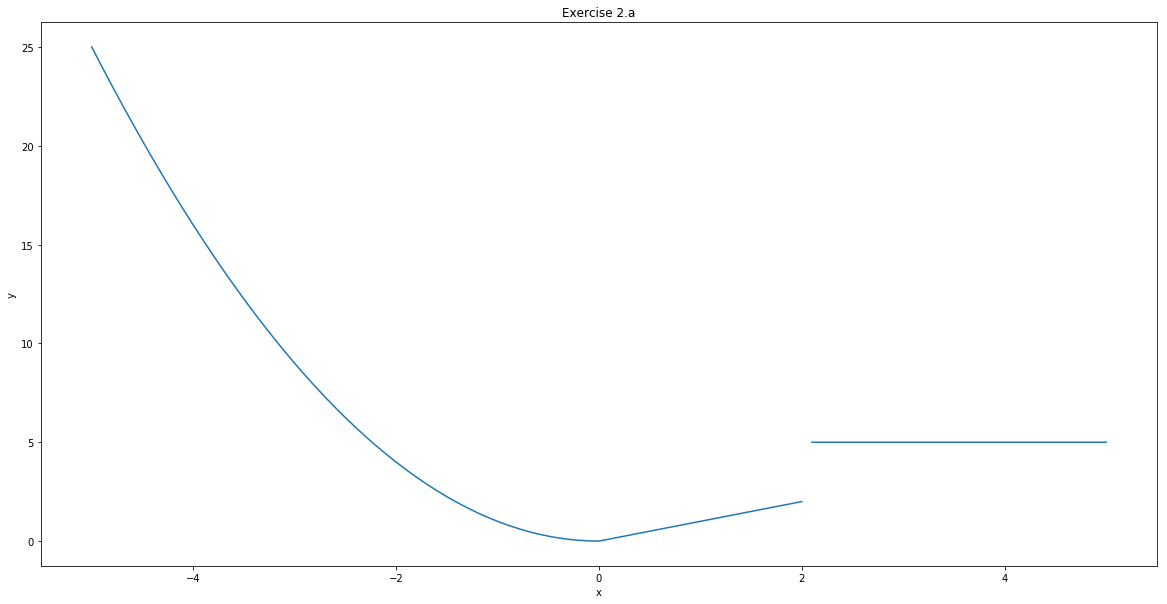
\includegraphics[width=\linewidth]{2a.png}
\end{center}
There is a single point in which the function is not continuous, in the point $x=2$, where the function jumps from $2$ to $5$.